\section{Refactoring} \label{sec:s4_refactoring}
%%% Intro paragraph --> Why do we refactor?

%%% How do we refactor?

%%% Summary --> Did the refactoring give us the desired results?

\subsection{class diagram}
\alnote{begrung UML}
\alnote{husk refere til uml standard}
In this section the model layer of the hotMap server's structure will be described, using a class diagram. The UML v2.5 standard for class diagram are mainly used for modeling the class diagram. The UML standard is not sufficient enough to represent all scala functionalities. In the static structure of the server application mixing is used which is a scala functionality that the UML standard cannot represent, so in order to represent mixing, realization arrows are used with a mixing stereotype.

Scala does not have interfaces, but instead uses traits. These are similar but allow for default implementation of methods. When a class implements an interface,  


In scala it's not possible to make interfaces, but instead there are trait's which essentially is the same as a interface except it is possible to have a default implementation of a method in a trait. Traits in scala also have the ability to inherit from classes, which usually does not apply for interfaces. When classes implement methods required by an interface, in the UML v2.5 standard this is called realization for traits.

Mixing means that a class or trait should realize more than one specific trait. This is illustrated by drawing two realizations arrows with the stereotype mixing, from the class to the traits. In \cref{fig:class} $Point$ is a mixing of $Coordinate$ and $Weight$, which means that the type $Point$ referees to a class which realises both $Coordinate$ and $Weight$. As seen on \cref{fig:class} there are no types which realises theirs class, so in order to construct a $Point$ a class inheriting from Coordinate implements the required method from the trait $Weight$ at instantiation time of the class.

\begin{figure}[!htb]
\centering
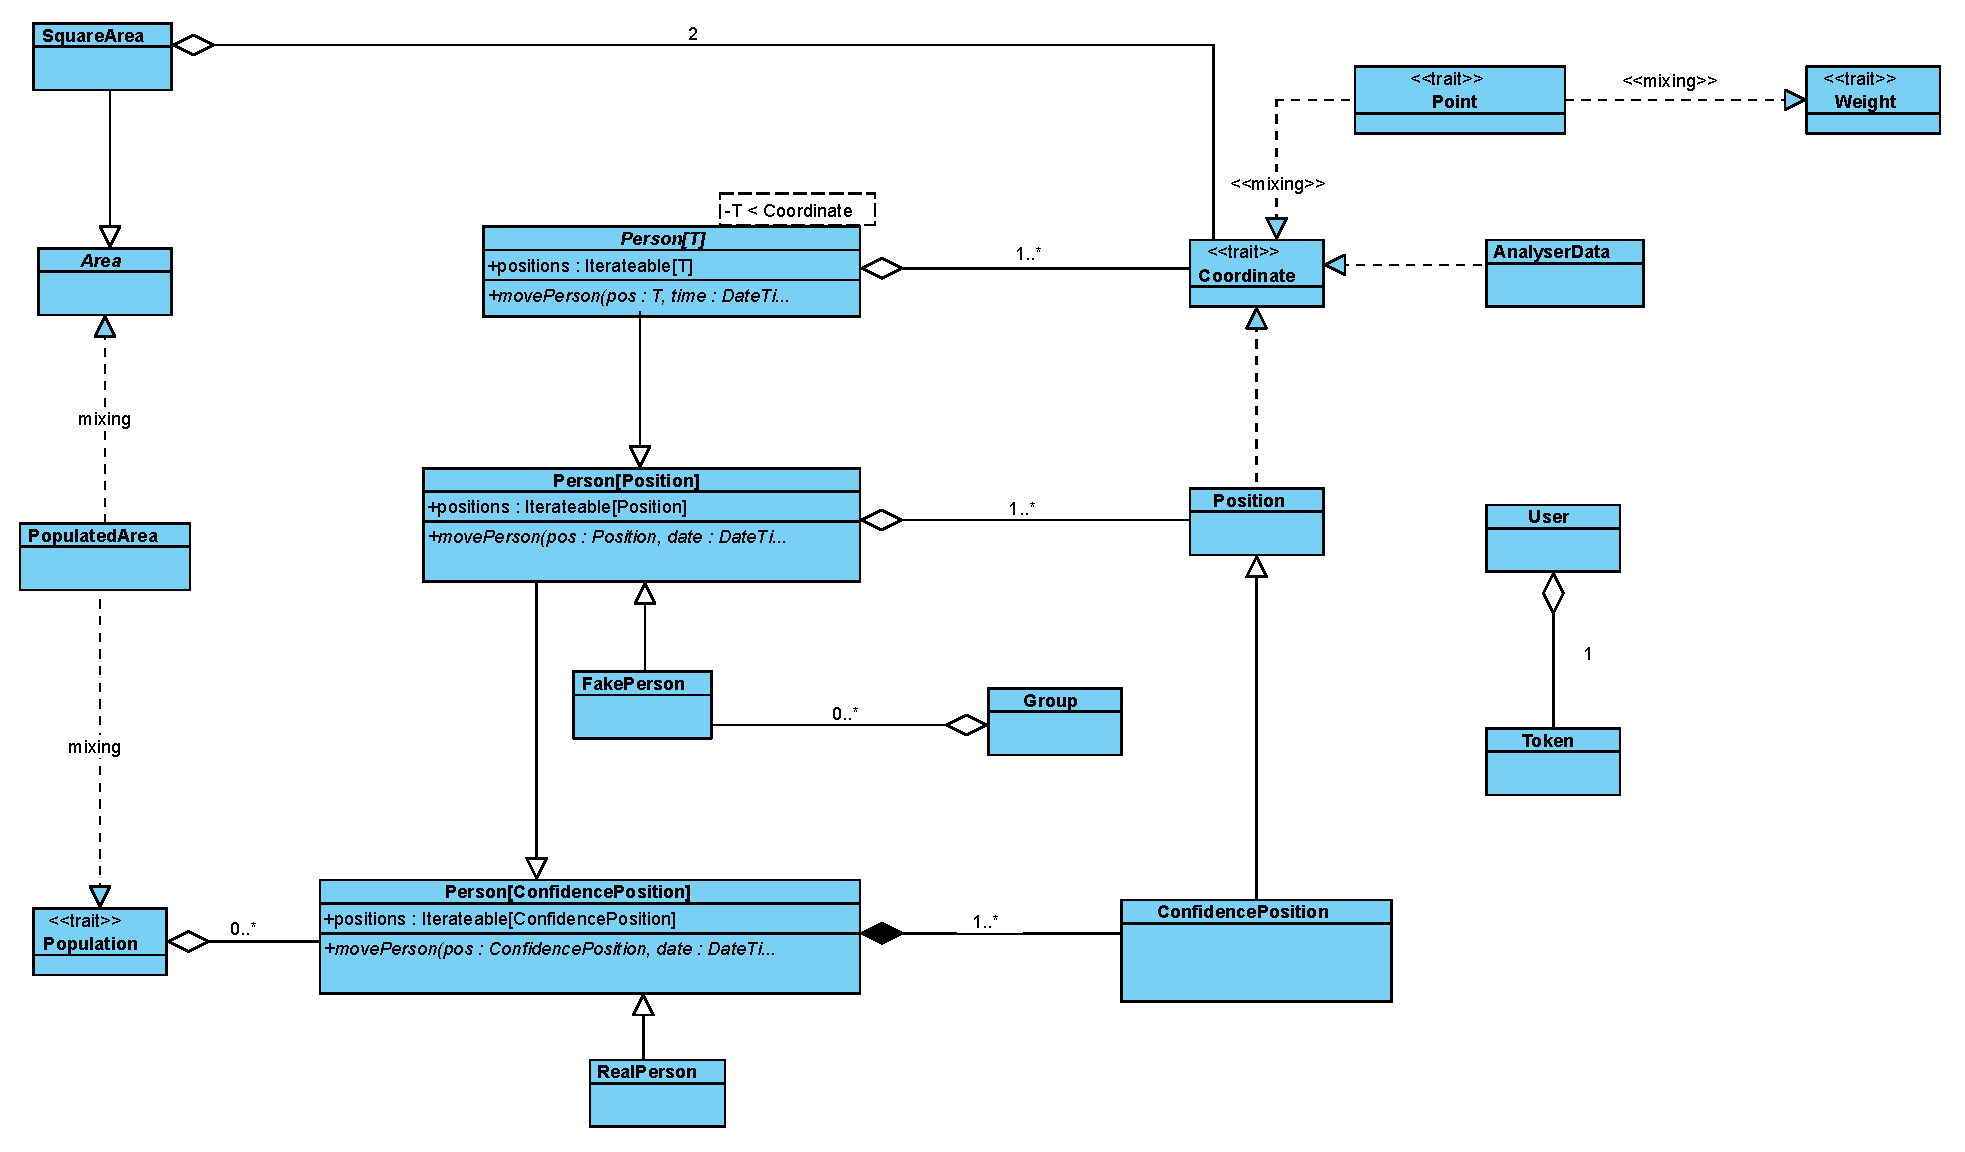
\includegraphics[scale=.7]{figures/class.eps}
\caption{Digraph.}
\label{fig:class}
\end{figure}